% LatexEx1.tex - Project 5 MAS6001

\documentclass[a4paper, 12pt]{report}

\usepackage[utf8]{inputenc}
\usepackage{amsmath}
\usepackage{amssymb}
\usepackage[super]{natbib}
\usepackage{graphicx}
\usepackage{epstopdf}
\usepackage[margin=1.0in]{geometry}
\usepackage{dcolumn}
\usepackage{appendix}
\usepackage{fixltx2e}	
\usepackage{natbib}
\usepackage{subfig}
\usepackage{float}
\usepackage{url}
\usepackage[nonumberlist]{glossaries}
\usepackage{setspace}
\usepackage[usenames, dvipsnames]{color}
\usepackage{titlepic}
\usepackage{standalone}
\usepackage{listings}

\onehalfspacing
\renewcommand{\abstractname}{Abstract of Measuring Non-linear Associations}
\makeglossaries
 %   \bibpunct[, ]{(}{)}{;}{a}{,}{,}

\title{Measuring Non-Linear Associations}
\author{Julian Roche  \\  \\ School of Mathematics and Statistics \\ \\ University of Sheffield}
\date{September 2015}

\newglossaryentry{A}
{
  name=A,
  description={A measure of association that generalises $R^2$ to handle non-linear associations. It is implemted in the R $matie$ package.}
}

\newglossaryentry{MATIE}
{
  name=MATIE,
  description={Measuring Association and Testing Independence Efficiently, an implementation in R of $A$}
}

\newglossaryentry{FDR}
{
  name=FDR,
  description={False Discovery Rate. A technique for limiting Type I errors in hypothesis tests}
}

\newglossaryentry{GAM}
{
  name=GAM,
  description={Generalised Additive Model}
}

\newglossaryentry{MARS}
{
  name=MARS,
  description={Multiple Adaptive Regression Splines}
}

\newglossaryentry{FDA}
{
  name=FDA,
  description={Flexible Discriminant Analysis}
}

\newglossaryentry{DE}
{
  name=DE,
  description={A gene which is differentially expressed}
}

\newglossaryentry{RV}
{
  name=r.v.,
  description={Random Variable}
}


\newglossaryentry{Equatibility}
{
  name=Equatibility,
  description={The ability to score equally, noisy relationships of different types}
}

\newglossaryentry{Power}
{
  name=Power,
  description={The ability to correctly reject the null hypothesis when it is false}
}


\newglossaryentry{MIC}
{
  name=MIC,
  description={Maximal Information Coefficient. An information theoretic measure of association}
}

\newglossaryentry{dcor}
{
  name=dcor,
  description={Distance correlation. A statistical measure of distance based on functions of distances between statistical observations in metric spaces}
}

\newglossaryentry{MDS}
{
  name=MDS,
  description={Multidimensional Scaling}
}

\newglossaryentry{AUC}
{
  name=AUC,
  description={Area under the curve}
}

\newglossaryentry{ROC}
{
  name=ROC,
  description={Receiver Operating Characteristic}
}


\newglossaryentry{Generality}
{
  name=Generality,
  description={The ability to detect departures from independence given a suffiiciently large sample}
}

\newglossaryentry{Pearson}
{
  name=Pearson's Correlation Coefficient,
  description={Represents the strength and direction of the linear correlation of two variables}
}

\newglossaryentry{Partial}
{
  name=Partial Correlation,
  description={}
}

\newglossaryentry{Spearman}
{
  name=Spearman's Rank,
  description={A non-parametric measure of dependence between two variables}
}

\newglossaryentry{Kendall}
{
  name=Kendall's Tau,
  description={A rank based measure of correlation}
}

\newglossaryentry{Spline}
{
  name=Spline,
  description={A numeric function composed of piecewise-defined polynomial functions}
}

\newglossaryentry{LDA}
{
  name=LDA,
  description={Linear Discriminant Analysis}
}

\newglossaryentry{PCA}
{
  name=PCA,
  description={Principal Component Analysis}
}

\newglossaryentry{Lupus}
{
  name=Lupus,
  description={An autoimmune disease of genetic origin}
}

\newglossaryentry{SLE}
{
  name=SLE,
  description={Systematic Lupus Erythematosus, see Lupus}
}

\newglossaryentry{Control}
{
  name=Control,
  description={Non-lupus patients}
}

\newglossaryentry{GE}
{
  name=Gene Expression,
  description={A measure of how a particular gene is expressed biologically}
}

\newglossaryentry{Correlation}
{
  name=Correlation,
  description={A statistical relationship between two random variables measuring how they vary with each other}
}

\newglossaryentry{Association}
{
  name=Association,
  description={A relationship between two variables describing their statistical dependence}
}

\newglossaryentry{Dependence}
{
  name=Dependence,
  description={A statistical relationship between two datasets}
}

\newglossaryentry{BD}
{
  name=Big Data,
  description={ Not strictly defined but typically refers to large, complex datasets that are too big to be managed using traditional methods. Examples of big data within pharmaceutical research include gene expression data, medical histories and clinical trial data}
}
\graphicspath {{../graphs/}}

\begin{document}
\pagestyle{myheadings}
 \markright{Julian Roche: Measuring Non-Linear Associations}

\maketitle

\pagenumbering{roman}

\begin{abstract}
\subsubsection*{Author: Julian Roche}
\subsubsection*{Date: September 2015}


This study compared three different measures of association (a probabilistic measure of association called $A$, distance correlation ($dcor$) and Maximal Information Coefficient ($MIC$)) at identifying inter-variable relationships in large biological datasets. The comparisons are based on power simulationsof two-way associations using a range of sample sizes, sampling distributions and additive noise levels.

The simulations found that no measure of association had greater statistical power in all cases. Using the gene expression data, $dcor$ identified all strong associations identified by $A$ in the two-way case. The analysis suggests that $A$ suffers from some of the same power deficiencies that have been previously identified for $MIC$.  

\end{abstract}

\newpage

\tableofcontents{}
 
\chapter{Introduction}
\pagenumbering{arabic}

\section{Motivation}
\gls{BD} is a fashionable term currently sweeping through the corporate world. While not strictly defined, it typically refers to large, complex datasets that are too big to be managed using traditional methods. Depending on the definition different statistical and computational challenges are posed. Examples of big data within pharmaceutical research include gene expression data, medical histories and clinical trial data. Often these have many more parameters than observations so $p >> n$. The availability of these datasets combined with recent developments for identifying associations between variables offers the potential to improve biological understanding which can in turn aid in the development of treatments for different diseases. 

%The term \gls{BD} has many definitions and is context dependent.  In this case the primary interest is in large biological datasets which typically have many more parameters than observations so the primary statistical challenge is to develop efficient methods for exploring very large numbers of relationships in relatively small sample sizes. 

One of the main purposes of association analysis is to produce an ordered list of variable pairs ranked by the strength of association. Typically these would form the basis of a more in-depth statistical analysis or highlight areas for further investigation or experimentation. The size of the datasets raises challenges for exploratory association mining. For example, when investigating $n$ pairwise combinations of variables there are $\frac{1}{2} \times n \times (n-1)$ combinations so that even for a dataset of 100 variables, there are 4095 different pairs to be analysed. 

A desirable property of estimators of association is that they can identify a range of different functional relationships equally and not for example be limited to just linear relationships, as is the case with Pearson correlation. % identify different types and strengths of non-linear relationships equally without biasing for particular types of relationships 
This has been highlighted as a potentially useful approach for studying gene expression where relationships may be determined by multiple distant factors  \cite{bigdata2012}. It is also important that different measures of association have sufficient statistical power when dealing with relatively small sample sizes. The situation becomes more complex when investigating multivariate associations or controlling for specific variables. Therefore automated, robust and efficient approaches to searching very large collections of variables are needed.

\section{Objectives}
The objective of the project is to compare three different measures of association ($A$, distance correlation ($\gls{dcor}$) and Maximal Information Coefficient ($\gls{MIC}$) at identifying inter-variable relationships and use these to develop efficient methods for analysing relationships in large biological datasets. The comparisons are based on simulated data and two gene expression datasets comparing lupus patients (see Section 1.5) with controls: a subset of genes deemed to be of biological interest (referred to as the training dataset) and a full Affymetrix chip (referred to as the test dataset)

\section{Overview}
Chapter 2 introduces the association measures studied and briefly reviews the concepts of dependence, association and non-linearity. Chapter 3 reports the results of a simulation study used to investigate the power of different association measures to detect dependence for a variety of functional relationships using various amounts of noise and sample sizes. Chapter 4 discusses the analysis and provides suggestions for further work. The Appendices provide ancillary material and code.



\chapter{Association and Non-Linearity}

\subsection*{Background}
%This section briefly introduces the concepts of random variables, dependence and association.
%
%A random variable can be defined as a real-valued function of an experimental outcome \cite{ITP}. A discrete random variable has a probability mass function giving the probability of each value which the random variable can take. A continuous random variable has a Probability Density Function (PDF) such that: 
%
%\[
%P(X \in B) = \int_B f_{X}(x) \,dx 
%\] 
%
%%A function of a random variable is also a random variable. The main interest in this study is in continuous random variables. 
%Two continuous random variables are jointly continuous when they are associated with the same experiment. They can be described in terms of their joint PDF, which is a positive function satisfying:  
%
%\[
%P((X,Y) \in B) = \iint_{(x,y) \in B} f_{X,Y}(x,y) \,dx \,dy
%\] 
%
%
%The joint PDF enables the calculation of the probability of any event involving the two random variables. The marginal PDFs of $X$ and $Y$ and can be obtained using the formulas:  
%
%\[
% f_X(x) = \int_{-\infty}^{\infty} f_{X,Y}(x,y) \,dy 
%\] 
%
%and
%
%\[
% f_Y(y) = \int_{-\infty}^{\infty} f_{X,Y}(x,y) \,dx 
%\] 
%
%The joint PDFs of multiple r.v.'s extends naturally, for example the joint PDF of three r.v.s $X$, $Y$ and $Z$ is given by:
%
%\[
%P((X,Y,Z) \in B) = \iiint_{(x,y,z) \in B} f_{X,Y,Z}(x,y,z) \,dx \,dy \,dz
%\] 

A linear function of two random variables is one that can be written in the form:

\[
y = ax + b
\]

where a and b are constants. Thus a non-linear function is a relationship which cannot be written as a linear combination of the the variables. Some examples of nonlinear functions are given and explored through simulation in Chapter 3.

If no relationship exists between two random variables they are said to be statistically independent. Formally, two events $A$ and $B$ are defined to be independent if:

\[
P(A \cap B) = P(A)P(B)
\]
 
Conversely, if two random variables $X$ and $Y$ are dependent then as $X$ changes in value, the value $Y$ will also change and vice versa. Association measures the statistical dependence between two of more random variables. In the case of two random variables this is a symmetric relationship.

\section{Measures of \gls{Association} }
There are many different statistics used to measure the association between random variables. A full comparison of all of these is obviously not practical so the measures explored through simulation and on the lupus datasets are introduced here. Other measures of association which are potentially of interest include mutual information and the Heller, Heller and Gorfine (HHG) measure \cite{HHG}. By convention association is measured on a $0-1$ scale, $0$ implying independence and $1$ implying complete dependence. \gls{Correlation} is also a measure of association but additionally includes the direction of the relationship between two random variables.

\subsection*{Generality and Equitability}
Two potentially desirable properties of measures of association, introduced by \citet{mic2011}, are:

\begin{itemize}
\item \gls{Generality}: The ability to detect any departure from independence given a suffiiciently large sample.
\item Equitibility: The ability to assign similar values of association to equally noisy relationships of different types.
\end{itemize}

The equitability property is of particular interest in large scale association studies as it offers the potential to efficiently search for pairwise relationships of different types in large datasets. It has attracted considerable interest in the context of biological studies \cite{bigdata2012} as a heuristic approach to discovering associations of interest. However, the property has also drawn criticism due to the fact that unless the measure has sufficient statistical power, inflated false discovery may reduce the utility of a given measure of association despite the equitability property \cite{Tibshirani2011}. Subsequent work by Kinney \cite{Kinney19082014}, which established a mathematical foundation for equitability based on $R^2$, suggests that $R^2$ equitability cannot be satisfied by any measure of association and therefore offers little practical value in exploratory analysis. However they introduced the notion of `self-equibality' which is falsifiable and therefore offers a way to compare measures of association. Kinney \cite{Kinney19082014} proved that $MIC$ is not self-equitable but that an information theortic measure called mutual information is and hence has potential for large scale association studies.


\subsection*{Pearson Correlation}
The Pearson correlation coeffiecent, $\rho$, measures the strenth and direction of a linear association between two r.v.'s, $X$ and $Y$. It is defined as

\[
\rho = \frac{cov(X,Y)}{\sigma_X \sigma_Y}
\]

where $cov(X,Y)$ is the covariance between $X$ and $Y$ and $\sigma_X$ and $\sigma_Y$ are the standard deviations of $X$ and $Y$ respectively.

The sample correlation coefficient is estimated as follows:

\[
\hat{\rho} = \frac{\sum_{i=1}^n(x_i - \bar{x})(y_i - \bar{y})}{s_X s_Y}
\]

where $\bar{x}$ and $\bar{y}$ are the sample means and $s_X$ and $s_Y$ the sample standard deviations of $X$ and $Y$ respectively. $R^2$  is known as the coefficient of determination and measures the amount of observed variance explained by a function. In the case of a linear relationship between two variables, $R^2 = \rho^2$. When the form of the functional relationship between two variables is unknown, obtaining a value of $R^2$ is more challenging \cite{Murrel:2013:Online} and has led to the development of many other measures of association.

\subsection*{Spearman's Rank Correlation}
Spearman's rank correlation is a non-parametric measure of association of paired data. For two r.v.'s $X$ and $Y$, it is calculated by ordering the $x$'s and $y$'s separately and then calculating the differences $d$ in the rank order between the two \cite{MSA}. Therefore a Spearman correlation of $1$ means that $X$ and $Y$ are in the same order. When ignoring ties it is given by the following formula:

\[
\rho_s = 1-\frac{6 \sum_{i=1}^n d_i^2}{n(n^2-1)}
\]

While Spearman's rank can describe non-linear relationships better than Pearson's correlation, it has been shown to not be equitable \cite{mic2011}.


\subsection*{Maximal Information Coefficient}
Maximal Information Coefficient ($MIC$) is based on the concept that if two random variables, $X$ and $Y$ are associated, the association can be defined by drawing a grid on a scatterplot of $X$ vs. $Y$. An outline of the algorithm for calculating $MIC$ is as follows:

\begin{enumerate}
\item For each pair of r.v.'s $X$ and $Y$ find the grid between $X$ and $Y$ with the highest mutual information (a measure of the variables' mutual dependence).%A tuning parameter is to control the level of discretisation in this step.
\item Normalise the mutual information scores in order to allow fair comparison of grids (grid dimensions may differ between pairs).
\item The normalised scores form a characteristic matrix, the maximum of which is the $MIC$ score.
\end{enumerate}

The following formal definition of $MIC$ is from \citet{mic2011}: for a grid $G$, let $I_G$ denote the mutual information of the probability distribution induced on the cells of $G$, where the probability of a cell is proportional to the number of points bounded by the cell. $m_{x,y} = \frac{max(I_g)}{log(min(x,y)}$ where $m_{x,y}$ is the $(x,y)$-th entry of the characteristic matrix, and the maximum is taken for all $x$ by $y$ grids $G$. The $MIC$ score is then the maximum of $m_{x,y}$ ordered pairs $(x,y)$ such that $xy < B$, where $B$ is a function of the sample size (the default is $B=n^{0.6}$ but the performance of $MIC$ is sensitive to this tuning parameter).  $MIC$ is implemented in the R $minerva$ \cite{minerva} package.

%The resultant $MIC$ value is then regarded as a relative test statistic for comparing pairwise relationships in a particular dataset rather than a general measure of association between two variables. 

\subsection*{$A$}
$A$ is a probabilistic measure of association that generalises $R^2$. It has a number of attractive features that make it of potential interest for association analysis, in particular the fact that it is reported\cite{Murrel:2013:Online} to have greater power than other measures of association such as $MIC$ and $dcor$, it extends to the multivariate case (e.g. how $Y$ is associated with both $X$ and $Z$) and can also measure association while controlling for covariates (i.e. partial association, the association between $Y$ and $X$ while controlling for $Z$). Additionally it is also reported to be both general and equitable\cite{Murrel:2013:Online}.

In the case of simple linear regression $y = f(x) + \epsilon$, $R^2$ quantifies the amount of observed systematic variation, while the residuals are assumed to be Normally distributed around $f(x)$. $A$ is based on the following reformulation of $R^2$:

\[
R^2 = 1-\prod_i(\frac{P(x_i,y_i|null)}{P(x_i,y_i|alt)})^{\frac{2}{n}}
\]

which defines $R^2$ in terms of the probability density of the null and alternative models. In the case of $A$, $\hat{A}$ can be estimated if suitable models for the null and alternative hypotheses can be found. In practice this involves estimating the density at each point of the null and alternative models using kernel density estimation. The choice of null is taken to enforce independence so $P(X,Y)=P(X)P(Y)$, while the alternative is is allowed to be dependent. For a detailed technical description see \citet{Murrel:2013:Online}. For simplicity the remainder of this document refers to $\hat{A}$ as $A$ unless explicitly stated otherwise.  It is implemented in the R $matie$ \cite{matie} package.


%Technically $\hat{A}$ is an estimator of $A$ and calculations of $A$ for the same to random variable (\gls{RV}) may differ slightly (about 2 decimal places).  a hyperbolic correction that is made during the estimation

\subsection*{Distance Correlation}
Distance correlation aims to measure all types of dependence between two or more random variables \cite{energy2013}. For two random vectors $X$ and $Y$ of size $n$, $dcor$ is computed as follows:

\begin{enumerate}
\item Compute a distance matrix of all pairwise distances between samples of the $X$ variable.
\item Compute the corresponding distance matrix for the $Y$ variable.
\item Mean centre both distance matrices, giving two distance matrices, $A_{k,l}$ and $B_{k,l}$, where $k$ and $l$ are the respective row and column indices.
\item Calculate the distance covariance: $dcov(X,Y) = \sqrt{\frac{1}{n^2} \sum^n_{k=1,l=1}A_{k,l}B_{k,l}}$.
\item Scale the distance covariance to give the distance correlation: \newline
$dcor(X,Y) = \frac{dcov(X,Y)}{\sqrt{dcov(X,X)dcov(Y,Y)}}$
\end{enumerate}

$dcor$ is implemented in the R $energy$ \cite{energy} package.  

\section{Assessing Non-Linearity}

The three association measures $MIC$, $A$ and $dcor$ all aim to measure all types of dependence, linear and non-linear, monotonic and non-monotonic etc. between pairs of random variables equally, however none explicitly measures the non-linear association. 
There are a number of possible ways of trying to assess the amount of non-linear association by partitioning the observed association into linear and non-linear components. \citet{Murrel:2013:Online} implement the following different measures of non-linearity based on $A$ and $R^2$ in the $matie$ R package \cite{matie}. They have been generalised here so that $\theta$ refers to any association measure.

\begin{enumerate}
\item Residual association ($r \theta$), the association of random variables after the linear relationship has been regressed out using a standard linear model. (See also \citet{energy2013}.) %This is an asymmetric relationship, hence $\thetaA(X,Y) \neq r\theta(Y,X)$. 
\item Difference, the non-linear part of the association, $\theta - R^2$. (See also \citet{mic2011}.)
\item The non-linear proportion of association, $\frac{(\theta-R^2)}{\theta}$
\item The proportion of total variance that is explained by $\theta$ but not by $R^2$, $\frac{(\theta-R^2)}{1 -\theta^2}$.
\end{enumerate}

\chapter{Simulation}

\section{Introduction}
Simulation was used to study a number of measures of association. The aim was to assess their utility and limitations for use in exploratory association mining in general and for the lupus dataset in particular. The analysis focused on how the statistical power of each association measures varies with noise and sample size.

Statistical power refers to the ability to identify correctly the null hypothesis when it is true. In the case of dependence the hypothesis is that two or more sets of data are independent while the alternative hypothesis is that they are dependent. Formally, for two random variables $X$ and $Y$: 
 \newline

$H_0$: $X$ and $Y$ are independent.

$H_1$: $X$ and $Y$ are dependent.
\newline

A previous simulation study by \citet{Tibshirani2011} into the power of $MIC$ vs. $dcor$ found that in most cases $dcor$ was more powerful than $MIC$ and that in the linear case $MIC$ was less powerful than \gls{Pearson}. This power deficiency led the authors to advocate the use of $dcor$ over $MIC$ in large scale exploratory analysis as $MIC$ might lead to too many false positives \cite{Tibshirani2011}. 

This simulation study extends the aforementioned study by including the $\gls{A}$ score, expanding the range of functional relationships explored, studying the effect of differing sample size and also using two source distributions. 

The original study used a \textit{Uniform(0,1)} to generate data which were then used to create dependent and independent sets of random variables $X$ and $Y$. The procedure is as follows: 

Let $X$, $Y$ and $Z$ be random variables and let $f(X)$ be a function of interest. For the dependant data: $X\sim U(0,1)$ and $Y = f(X)$. For the independent data: $X\sim U(0,1)$, $Z\sim U(0,1)$  and $Y = f(Z)$.


Their motivation for choosing \textit{Uniform(0,1)} distribution was primarily because the authors of $MIC$ had used it in their simulation studies\cite{Tibshirani2011, mic2011}. Exploratory analysis of the lupus dataset suggested that many of the gene expressions have positively skewed distributions, so a \textit{Beta(2,5)} distribution was used to simulate this. 

The main interest was in comparing $\gls{A}$, $MIC$ and $dcor$.  Pearson and Spearman correlation were also included for contrast. Fifteen different functional relationships were studied. The functions are defined in Table \ref{T:functions}. Normally distributed noise was added to each function so that, $y = f(x) + l \times \epsilon$, where $l$ is a scaling parameter controlling the level of noise, $\epsilon$, and $\epsilon \sim N(0, 1)$. In the case of the cubic, exponential, log, step, spike and sine based functions, $l$ was scaled to compensate for the range of $y$. Figure \ref{F:FunctionForms} plots each of these for a sample size of 320 with minimal noise.


\begin{table}[h]
\centering
\begin{tabular}{ll}
  \hline
Name & Function  \\ 
  \hline
Linear &  $y = x$ \\ 
 Quadratic &  $y=4(x-\frac{1}{2})^2$ \\ 
  Cubic &  $y = 128(x-\frac{1}{3})^3 -48(x-\frac{1}{3})^3 -12(x-\frac{1}{3}) $\\ 
  Fourth Root &  $y = x^{\frac{1}{4}}$ \\ 
  Exponetial &  $y = e^{x^2}$ \\ 
  Log &  $y = ln(x)$ \\ 
  Sigmoid &  $y = 1 + e^{10(\frac{1}{2}-x)^{-1}}$ \\ 
  Step &   $
y =
\begin{cases} 
+1 &\text{when } x \ge 0.5\\
-1 &\text{otherwise} \\
\end{cases}$\\ 
  Spike &  $
y =
\begin{cases} 
4 &\text{when } x \le 0.05\\
1.9 -18x &\text{when } x \le 0.10\\
\frac{1}{9} - \frac{x}{9}&\text{otherwise} \\
\end{cases}$ \\ 
  Sine: Low &  $y = sin(4 \pi x)$  \\ 
  Sine: High  &  $y = sin(16 \pi x)$  \\ 
  Linear + Periodic &  $y = x +  sin(10 \pi x)$  \\ 
  Varying Frequency &  $y = x +  sin(5 \pi \frac{1}{x})$  \\ 
  Circle &  $y = (1 - (2x -1)^2) \times -2z$, where $Z \sim B(1,\frac{1}{2})$ \\ 
  X &  $y = 4(x-\frac{1}{2})^2 \times z$, where $P_Z(z)= \begin{cases} 
\frac{1}{2} &\text{when } z = +1\\
\frac{1}{2} &\text{when } z = -1\\
\end{cases}$ \\ 
   \hline
\end{tabular}
\caption{The fifteen functions being evaluated.} 
\label{T:functions}
\end{table}

\begin{figure}[H]
\begin{centering}
\includegraphics[width=\textwidth]{FunctionFormsNoNoise.pdf}
\caption{Scatter plots showing the fifteen different functional forms being evaluated. } 
\label{F:FunctionForms}
\end{centering}
\end{figure}


\section{Power versus Noise}
In order for an association measure to be practically useful in association analysis it should have reasonable statistical power for noisy data. Ideally it should also be equitable, i.e. it should score equally different types of relationships with equal amounts of noise added. This simulation explored how statistical power varied for the different functional forms for different amounts of Normally distributed noise. A sample size of 320 was used to represent a moderately size biological dataset. (Figure \ref{F:FunctionFormsNoise} in Appendix A shows each functional form following the addition of noise.) 

Data was generated using two  distributions, \textit{Uniform(0.1)} and \textit{Beta(2,5)}, so for a  r.v. $X$, $X \in \{0,1\}$. Random noise was generated from a $N(0,1)$ distribution and then scaled by a given noise level (0.1 to 3). The following algorithm was used in the simulation to assess if two r.v.'s $X$ and $Y$ were dependent:

%$H_0$: $X$ and $Y$ are independent.

%$H_1$: $X$ and $Y$ are dependent.

%The simulation algorithm is as follows:
 
\begin{enumerate}
\item For each functional form, $f$, and noise level, $l$:
\item Generate independent r.v.'s $X,Y$ and $Z$: $X$ and $Z$ from the given distribution (so $X \in \{0,1\}, Z \in \{0,1\}$) and an independent r.v. $Y=f(Z) + l \times \epsilon$, where $\epsilon \sim N(0,1)$.
\item Measure the association between $X$ and $Y$ using $A$, $dcor$, $MIC$, $\rho_{pearson}^2$ and $\rho_{spearman}^2$
\item Generate dependent r.v.'s $X$ and $Y$: $X$ from the given distribution and a dependent r.v. $Y=f(X) + l \times \epsilon$, where $\epsilon \sim N(0,1)$. 
\item Measure the association between $X$ and $Y$ using $A$, $dcor$, $MIC$, $\rho_{pearson}^2$ and $\rho_{spearman}^2$
\item Estimate the power as the number of times the association score for the dependent data exceeds the $95^{th}$ percentile of the corresponding score for the independent data.
\item Repeat $500$ times.
\end{enumerate}

The complete $R$ code, based on that of \citet{Tibshirani2011}, is given in Appendix A. The results in Figure \ref{F:powerNU} suggest that all measures are sensitive to the level of noise and that none of the measures has greater power for all of the functional forms simulated. In particular $A$ appears to have low power for the fourth root, step, exponential, sigmoid and linear cases. It also has lower power than $dcor$ in the cubic cases. Both $A$ and $MIC$ generally outperform $dcor$ for periodic functions most notably for the high frequency sine wave. Interestingly, $A$ has the highest power in detecting the circle and `X' shapes.
%This suggests that $A$ may have limited usefulness as a measure of association for exploratory analysis depending on how noisy the dataset appears to be and depending on which (if any) functional form is being investigated. 

Simulation results from the skewed distribution were broadly similar to that shown in Figure \ref{F:powerNU} are given in Appendix A.2 (Figure \ref{F:powerNB}). For most functional forms there was a decrease in power, most notably for the step function which showed a reduction in power for all association measures. Both $A$ and $MIC$ also had lower power than Pearson correlation in the quadratic and cubic cases.
%Spearman and Pearson correlation have similarly low power in non-linear settings.

\begin{figure}[H]
\begin{centering}
\includegraphics[width=\textwidth]{powerNoiseUN.pdf}
\caption{Scatter plots showing the power of each measure of association vs. noise for each functional form based on 320 observations from a $Uniform(0,1)$ distribution.} 
\label{F:powerNU}
\end{centering}
\end{figure}

\section{Power versus Sample Size}
Typically for biological datasets the sample size, $n$, is relatively small (in the case of the lupus dataset $n = 420$), while $n > 1000$ would generally considered a large dataset. Hence to be of practical use an association measure should be sufficiently powerful at detecting associations on small datasets. This was the objective of this simulation.  

An adapted version of algorithm given in the previous section was used to explore how power varies with sample size in the presence of moderate noise:

\begin{enumerate}
\item For each functional form, $f$, and sample size, $n\in$ \{10, 20, 30, 40 ,50, 75, 100, 125, 150, 200, 250, 300, 350, 400, 500, 750, 1000\}:
\item Generate independent r.v.'s $X,Y$ and $Z$: $X$ and $Z$ from the given distribution (so $X \in \{0,1\}, Z \in \{0,1\}$) and an independent r.v. $Y=f(Z) + l \times \epsilon$, where $l=1$ and $\epsilon \sim N(0,1)$
\item  Measure the association between $X$ and $Y$ using $A$, $dcor$, $MIC$, $\rho_{pearson}^2$ and $\rho_{spearman}^2$
\item Generate dependent r.v.'s $X$ and $Y$: $X$ from the given distribution and a dependent r.v. $Y=f(X) + l \times \epsilon$, where $l=1$ and $\epsilon \sim N(0,1)$. 
\item  Measure the association between $X$ and $Y$ using $A$, $dcor$, $MIC$, $\rho_{pearson}^2$ and $\rho_{spearman}^2$
\item Estimate the power as the number of times the association score for the dependent data exceeds the $95^{th}$ percentile of the corresponding score for the independent data.
\item Repeat $500$ times.
\end{enumerate}

Again the algorithm was run with a \textit{Uniform(0,1)} distribution and then with a \textit{Beta(2,5)} distribution to see if a skewed source distribution affected the results. The results for the \textit{Uniform} case are given in Figure \ref{F:powerSizeUN10}. The results show that $A$, $MIC$ and $dcor$ only converged in certain cases but that $dcor$ converged more quickly (i.e. is more powerful on smaller sample sizes) in the linear, quadratic, cubic and exponential cases. The power of $dcor$ was again noticeably low in the high frequency sine case. No measures converged for the step, spike, linear+periodic or varying frequency functions function. $A$ and $MIC$ both failed to converge for $X^{\frac{1}{4}}$.


\begin{figure}[H]
\begin{center}
\includegraphics[width=\textwidth]{powerSizeUN10.pdf}
\caption{Scatter plots showing the power of each measure of association vs. sample size using a $Uniform(0,1)$ distribution.} 
\label{F:powerSizeUN10}
\end{center}
\end{figure}

In the case of the skewed distribution, the performance of all measures generally declined, particularly for $A$ and $MIC$ in the quadratic and cubic cases. The power of $A$, $MIC$ and $dcor$ also reduced for the exponential function. The results are shown in Figure \ref{F:powerSB} in Appendix A.

Simulations were also run using the maximum level of noise and using a skewed distribution. The results are shown in Figure \ref{F:powerSizeBN30} in Appendix A.2 and show that none of the association measures were powerful at detecting dependence on very noisy relationships even when the sample size was large ($n=1000$).

\chapter{Discussion and Further Work}

The simulation studies focused on how the power of the different measures of association perform in the presence of noise and with different sample sizes. This is of particular relevance to biological datasets which can contain a large amount of technical variability which is not of interest and typically have small sample sizes but many dimensions. 

Unsurprisingly the simulations showed that in general power decreases in the presence of increasing noise while power increases with increased sample size even in the presence of noise. Of greater importance is that the analysis suggested that $A$ suffers from some of the same power deficiencies as $MIC$ for certain important cases such as linear and cubic but both surpass $dcor$ where high frequency periodic variation exists. This appears to confirm the reservations regarding the equitability heuristic expressed by \citet{Kinney19082014} and \citet{Tibshirani2011}. The size simulations questions the practical usefulness of the generality heuristic.

No one measure exceeded all of the others in all of the cases, however on balance the simulation study suggests that $dcor$ should perform better than either $MIC$ or $A$ on the basis of capacity to handle noise and deal with small sample sizes. From a practical perspective if the form of a relationships are unknown then $dcor$ would appear to be the best choice of association measure, possibly in conjunction with Pearson Correlation (to assess non-linearity) and either $A$ or $MIC$ if periodic effects are suspected or known a priori.

%The level of noise is a somewhat relative term but in a real dataset would not be known apriori meaning that a test statistic such as $dcor$ would be preferred over either $MIC$ or $A$. 

There are many other simulation based analyses that could be performed. The noise and size studies both held either size or noise constant, an obvious extension would be to allow both noise and sample size to vary simultaneously to get a more complete power profile.  Further extensions would be to expand the range of functional forms and source distributions and to include three way and partial associations where possible. Additionally it would be of interest to explore  relative performance of $HHG$ \cite{HHG} which has been identified as being of potential use for exploratory association mining. 

The goal of the analysis was to compare the relative of abilitity different measures of association to estimate extant non-linear relationships. 

Association analyses are essentially exploratory in nature and provide no evidence of causation. There are numerous sources of technical and biological variation which might be responsible for observed associations. In reality the results of an association analysis would serve as the basis for a more refined follow on study or, if the goal is to establish causality, a suitably designed controlled experiment. 

Of the measures of association studied, on balance, $dcor$ had better performance than either $A$ or $MIC$ on the lupus data in terms of associations identified. The simulations suggest that $dcor$ generally has greater power with small sample sizes and noisy datasets but that $MIC$ and $A$ have greater power for certain functional types. Knowing the relative strengths and weaknesses of each measure is a critical aspect to choosing which association to use. The  choice of which to use might depend on the types of functional relationships suspected to exist in the data or to the extent of the computational resources available. A pragmatic option is to combine a number of measures such as $dcor$ and $A$ and use the knowledge of the measures' properties to critically evaluate the results obtained.

There are many other measures of association that could be compared, most notably mutual  information and the Heller-Heller-Gorfine \cite{HHG} measure. Another extension would be to investigate partial associations, i.e. measuring the strength of association while one variable is controlled for. There also a number of alternative methods that can be used to assess inter-variable association and whether or not it can be best described linearly or non-linearly. Two Bayesian approaches to this are an R package called $spikeSlabGAM$ \cite{spikeSlabGAM} and another approach presented by \citet{BayesianGRN} which would make an interesting comparison in a future study. 

 A further extension would be to study the sensitivity of both $A$ and $dcor$ to their respective tuning parameters. The bootstrap estimates of both $MIC$ and $A$ appeared to converge more closely with $dcor$ than their point estimates. This could also be studied through simulation however even if the accuracy improves, the added computational overhead might render it impractical.



\bibliographystyle{unsrtnat}
\bibliography{refdatabase}

\printglossary

%%%%%%%%%%%%%%%%%%%%%%%%%%%%%%%%%%%%%%%%%%%%%%%%%%%%
%%%%%%%%%%%%%%%%%%%%%%%%%%%%%%%%%%%%%%%%%%%%%%%%%%%%
\appendix

\chapter{Additional Results}


\section{Simulation Results}

\begin{figure}[H]
\begin{centering}
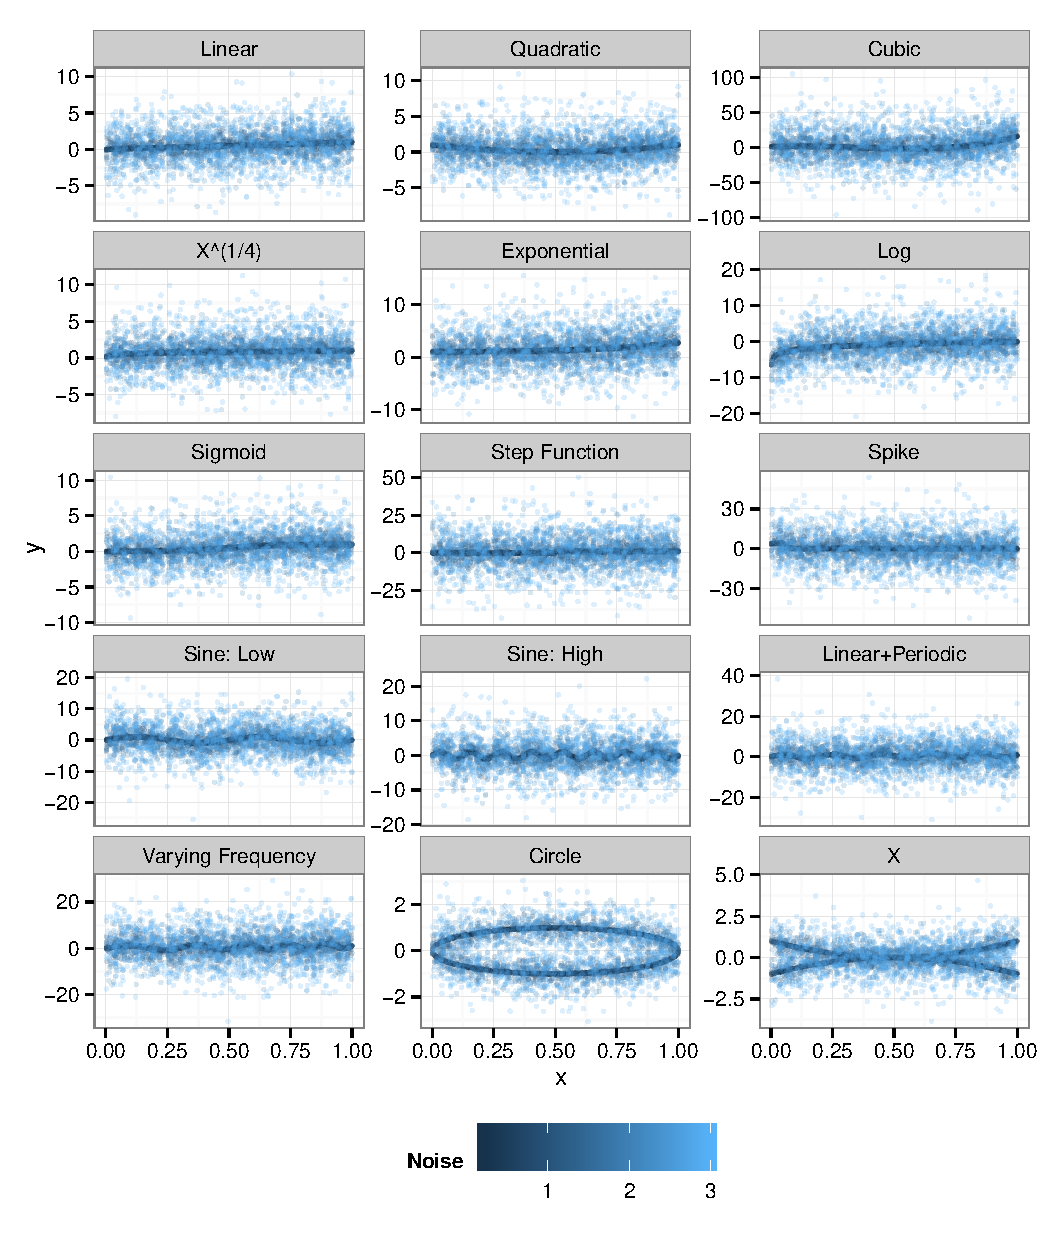
\includegraphics[width=\textwidth]{forms.pdf}
\caption{Scatter plots showing the fifteen different functional forms with varying amounts of random noise. In each plot the darkest points show the minimum noise added while the lighter points show increasing levels of noise. The differences in the y-axes reflect the differences in the range of $y$ for each function.} 
\label{F:FunctionFormsNoise}
\end{centering}
\end{figure}

\begin{figure}[H]
\begin{centering}
\includegraphics[width=\textwidth]{beta25Noise.pdf}
\caption{Scatter plots showing the power of each measure of association vs. noise for each functional form based on 320 observations from a $Beta(2,5)$ distribution. Note the reduction in power for the step function.} 
\label{F:powerNB}
\end{centering}
\end{figure}



\begin{figure}[H]
\begin{center}
\includegraphics[width=\textwidth]{powerSizeBeta25Noise10Final.pdf}
\caption{Scatter plots showing the power of each measure of association vs. size for each functional form based on a $Beta(2,5)$ distribution. For the exponential function the power reduced for $dcor$, $A$ and $MIC$.} 
\label{F:powerSB}
\end{center}
\end{figure}

\begin{figure}[H]
\begin{centering}
\includegraphics[width=\textwidth]{powerSizeNoise30Beta25.pdf}
\caption{Scatter plots showing the power of each measure of association vs. sample size for each functional forms. None of the measures converged.} 
\label{F:powerSizeBN30}
\end{centering}
\end{figure}






\end{document}